\documentclass[draft,11pt]{report}

% Packages {{{
\usepackage[margin=1in,left=1.5in]{geometry}
\usepackage{amsmath}
\usepackage{amssymb}
\usepackage{amsthm}
\usepackage{natbib}
\usepackage{tikz}
\usetikzlibrary{calc}
\usetikzlibrary{graphs}
\usetikzlibrary{cd}
\usetikzlibrary{patterns}
\usepackage{bbm}
\usepackage{soul}
\usepackage{ebproof}
\usepackage{stmaryrd}
\usepackage{setspace}
\doublespacing

% From CompCertO
%\usepackage{hyperref}
%\usepackage{galois}
%\usepackage{calc}
%\usepackage{booktabs}
%\usepackage{listings}
% }}}

% Macros {{{

\newtheorem{definition}{Definition}
\newtheorem{lemma}{Lemma}
\newtheorem{theorem}{Theorem}
\newtheorem{example}{Example}

\newcommand{\gcat}{\mathcal{G}_{\sqsubseteq}}
\newcommand{\kw}[1]{\ensuremath{ \mathsf{#1} }}
\newcommand{\ifr}[1]{\mathrel{[{#1}]}}
\newcommand{\ifrw}[2]{\mathrel{[{#2} \Vdash {#1}]}}
\newcommand{\bdot}{\boldsymbol{\cdot}}
\newcommand{\alt}{\mid} % update and remove
\newcommand{\plays}[4]{{ {#1}_{{#2} \rightarrow {#3}}[{#4}] }}
\newcommand{\pplays}[3]{\plays{\bar{P}}{#1}{#2}{#3}}
\newcommand{\oplays}[3]{\plays{P}{#1}{#2}{#3}}
\newcommand{\htr}[3]{{ {#1} \mathbbm{\{} {#2} \mathbbm{\}} {#3} }}
\newcommand{\sbt}{\,\begin{picture}(-1,1)(-1,-3)\circle*{3}\end{picture}\ }

\newcommand{\que}{\circ}         % superscript for questions
\newcommand{\ans}{\bullet}       % superscript for answers
\newcommand{\vref}{\le_\kw{v}}   % value refinement
\newcommand{\mext}{\le_\kw{m}}   % memory extension
\newcommand{\refby}{\preceq}     % refinement relation
\newcommand{\scref}{\sqsubseteq} % simulation convention refinement

% Moves {{{

\newcommand{\mcall}[3]{\kw{#1}({#2})@{#3}}
\newcommand{\pcall}[3]{%
  \underline{\mcall{#1}{#2}{#3}}%
}
\newcommand{\mret}[2]{{#1}@{#2}}
\newcommand{\pret}[2]{%
  \underline{\mret{#1}{#2}}%
}
\newcommand{\mretx}[3]{{#1}@{#2}/{#3}}
\newcommand{\pretx}[3]{%
  \underline{\mretx{#1}{#2}{#3}}%
}

% }}}

% Pointers for justified sequences %{{{

% Parameters
\newcommand{\pshift}{1.6ex}
\newcommand{\pcdist}{2.5}
\newcommand{\pcangle}{60}

% Pointer hook
\newcommand{\ph}[1]{%
  \tikz[remember picture]{\coordinate (#1);}}

% Pointer to
\newcommand{\pt}[1]{%
  \rule{0pt}{1.4em}%
  \tikz[remember picture, overlay]{
    \draw[->]
      let \p{dest} = (#1),
          \n1 = {ln(veclen(\x{dest}, \y{dest}) + 1)},
          \p1 = ($(0,0)+(0,\pshift)$),
          \p4 = ($(#1)+(0,\pshift)$),
          \p2 = ($(\p1)!\n1*\pcdist!-\pcangle:(\p4)$),
          \p3 = ($(\p4)!\n1*\pcdist!+\pcangle:(\p1)$) in
        (\p1) .. controls (\p2) and (\p3) .. (\p4);}}

%}}}

\hyphenation{Comp-Cert}
\hyphenation{Comp-CertO}
\hyphenation{Comp-CertX}
\hyphenation{Certi-KOS}

% }}}

\title{Refinement-based game semantics}
\author{J\'er\'emie Koenig}

\begin{document}

\begin{abstract}
%
\begin{abstract} % From rbgs-cal {{{
Formal methods have advanced to the point where
the functional correctness of various large
system components has been mechanically verified.
However,
the diversity of semantic models used across projects
makes it difficult to connect these component
to build larger certified systems.
%Therefore,
Given this,
we seek to embed these models and proofs
into a general-purpose framework
where they could interact. %be made interoperable.
%linked together to
%construct certified heterogeneous systems.
We believe that a synthesis of game
semantics, the refinement calculus, and algebraic effects can
provide such a framework.

To combine game semantics and refinement, we replace the downset
completion typically used to construct strategies from posets of plays.
Using the \emph{free completely distributive completion},
we construct \emph{strategy specifications}
equipped with arbitrary angelic and demonic choices
and ordered by a generalization of alternating refinement.
This provides a novel approach to nondeterminism in game semantics.

%To connect
Connecting algebraic effects and game semantics, we interpret effect
signatures as games and define two
categories %$\gcat^{ib}$ and $\gcat^b$
of effect signatures and strategy
specifications.
The resulting models are sufficient to represent the behaviors
of a variety of low-level components,
including the \emph{certified abstraction layers}
used to verify the operating system
kernel CertiKOS. %~\cite{popl15}.
\end{abstract}
%}}}

\begin{abstract} % From rbgs-compcert {{{
Since the introduction of CompCert,
researchers have been refining
its language semantics and correctness theorem,
and used them in
large-scale software verification efforts.
Meanwhile,
artifacts ranging from CPU designs to network protocols
have been successfully verified,
and there is interest in
making them interoperable
to tackle end-to-end verification
at an even larger scale.

To that end,
we believe that
a synthesis of existing research on
game semantics,
refinement-based methods, and
abstraction layers
has the potential to serve as a common theory
of certified components,
and that integrating CompCert to such a theory
is a critical goal.
However,
the requirements we have identified for
CompCert to be deployed in this context
are not met by any of its existing variants.

CompCertO is
a new extension of CompCert
which characterizes compiled program modules
in terms of their interaction with other components.
By extending the CompCert semantics
in a way that embraces relational reasoning,
we achieve this with only a minimal increase
in proof size.
\end{abstract}
%}}}


\end{abstract}

\titlepage

\tableofcontents

\chapter{Introduction}

\chapter{Background}

\chapter{Certified abstraction layers}

\chapter{Refinement-based game semantics}

\section{Refinement-based game semantics}

\subsection{Overview}



Games are identified with the type of moves.

\subsection{Alternating transition systems}

Strategies are specified using transition systems
alternating between a set of states $S$ and
a set of continuations $K$.
States correspond to points in the execution
where the system is expected to move,
whereas continuations expect a move from the environment
and specify how the execution should be resumed.

The initial configuration of the system
is specified by a continuation.
For each continuation $k \in K$
and each possible move $m \in M$ from the environment
we specify a set of possible \emph{resumptions}
among the following:
\[ r \in \kw{resumption}(S) ::=
	\kw{resume}(s) \ |\ \kw{refuse} \]
If the environment's input move is accepted,
the execution can proceed in state $s$.
Alternatively,
a continuation may \emph{refuse} a given input move,
as indicated by the resumption $\kw{refuse}$.
In the context of composite systems,
this will allow another component to proceed.

We associate to each state $s$ a set of possible
behaviors among the following:
\[ b \in \kw{behavior}(M,S,K) ::=
	\tau \cdot s' \ |\
	\underline{m} \cdot k \ | \
	\Delta \ |\ 
	\lightning \]
The behavior $\tau \cdot s'$
performs an internal action and transitions to state $s'$;
the behavior $\underline{m} \cdot k$
plays the move $m$ and transitions to the continuation $k$;
the behavior $\Delta$ represents silent divergence,
an indication that the system will no longer perform
any externally observable action;
$\lightning$ indicates that the system ``goes wrong''.

For simplicity, and without loss of generality,
in the following we will take the set of continuations
to be defined in terms of $S$ as:
\[ K := M \rightarrow \mathcal{P}(\kw{resumption}(S)) \,. \]

\begin{definition}[Alternating transition system]
For a set of moves $M$ and a set of states $S$,
an \emph{alternating transition system} is a relation:
\[
  \alpha : S \rightarrow \mathcal{P}(\kw{behavior}(M, S)) \,.
\]
The type of alternating transition systems on $M$ and $S$
will be written as $\kw{ats}(M, S)$.
\end{definition}

For clarity,
and to establish a connection with more typical
labelled transition systems,
we will write:
\begin{itemize}
\item $s \xrightarrow{\tau} s'$ whenever $\alpha(s) \ni \tau \cdot s'$;
\item $s \xrightarrow{\underline{m}} k$
	whenever $\alpha(s) \ni \underline{m} \cdot k$;
\item $s \xrightarrow{\lightning} {\cdot}$
	whenever $\alpha(s) \ni \lightning$,
	and similarly for $\Delta$;
\item $k \xrightarrow{m} r$ whenever $k(m) \ni r$.
\end{itemize}
These notations can be concatenated so that
we will write $x \xrightarrow{t \cdot t'} z$
whenever there exists $y$ such that $x \xrightarrow{t} y$ and
$y \xrightarrow{t'} z$.
For a given alternating transition system $\alpha$,
the set of traces associated with a state or continuations $x$
can be defined as:
\[
    \kw{traces}_\alpha(x) =
	\{ t \:|\: \exists y \,.\, x \xrightarrow{t} y \} \,.
\]

Strategies can be defined in terms of alternating transition systems
by providing an initial continuation and hiding the set of states.

\begin{definition}[Strategy]
For a set of moves $M$,
a strategy $\sigma = (S, \alpha, k_0)$
is a set of states $S$ together with
an alternating transition system $\alpha : \kw{ats}(M, S)$ and
an initial continuation $k_0 : S \rightarrow \mathcal{P}(\kw{resumption}(S))$.
\end{definition}

For a strategy $\sigma = (S, \alpha, k_0)$,
we define its set of traces as
$\kw{traces}(\sigma) = \kw{traces}_\alpha (k_0)$.

\subsection{Refinement conventions}

Given two strategies $\sigma_1, \sigma_2$,
we want to formulate a notion of refinement
$\sigma_1 \sqsubseteq \sigma_2$.
To make it possible to relate strategies at different
levels of abstraction,
we will need to specify how the moves of $\sigma_1$
relate to those of $\sigma_2$
as the execution proceeds.
since this is a stateful process,
we formalize this \emph{refinement convention}
as a Kripke logical relation between the two games.

\begin{definition}[Refinement convention]
Given two sets of moves $M_1$, $M_2$,
a refinement convention
is a Kripke logical relation $\mathbb{R} = (W, \leadsto, R_M)$
between $M_1$ and $M_2$.
\end{definition}

We obtain our notion of refinement by extending $\mathbb{R}$
in a natural way,
first to state behaviors and continuation resumptions,
then to simulations of transition systems,
and finally to our refinement of strategies.

\subsection{Simulations}

For a refinement convention $\mathbb{R} : \mathcal{R}_W(M_1, M_2)$,
a Kripke logical relation on states $R : \mathcal{R}_W(S_1, S_2)$
can be extended to resumptions as follows:
\[
  \AxiomC{$s_1 \ifr{w \Vdash R} s_2$}
  \UnaryInfC{$\kw{resume}(s_1) \ifr{w \Vdash R} \kw{resume}(s_2)$}
  \DisplayProof
  \qquad
  \AxiomC{\rule{0pt}{\baselineskip}}
  \UnaryInfC{$\kw{refuse} \ifr{w \Vdash R} \kw{refuse}$}
  \DisplayProof
\]
For simple state behaviors,
refinement is defined as follows:
\[
  \AxiomC{$s_1' \ifr{w \Vdash R} s_2'$}
  \UnaryInfC{$\tau \cdot s_1' \ifr{w \Vdash R} \tau \cdot s_2'$}
  \DisplayProof
  \quad
  \AxiomC{\rule{0pt}{\baselineskip}}
  \UnaryInfC{$\Delta \ifr{w \Vdash R} \Delta$}
  \DisplayProof
  \quad
  \AxiomC{\rule{0pt}{\baselineskip}}
  \UnaryInfC{$b \ifr{w \Vdash R} \lightning$}
  \DisplayProof
\]
Note that the behavior $\lightning$ is defined as a top element
for refinement,
so that a strategy that goes wrong can be refined arbitrarily
but can only implement a specification that
also goes wrong.
By contrast,
explicit divergence $\Delta$
is only related to itself,
and counts as a specific behavior on par with others.

For interacting state behaviors,
the KLR structure is going to come into play.
Two continuations $k_1, k_2$ are related when
for any world transition,
and any two moves which are related in the new world,
every resumption of $k_1$ has a corresponding resumption in $k_2$:
\[
  R_K := \Box (\mathbb{R} \rightarrow \mathcal{P}^+(R))
\]
Two interactions are related
if there exists a world transition that relates the output moves,
and relates the associated continuations:
\[
  \AxiomC{$(m_1, k_1) \ifr{w \Vdash \Diamond (\mathbb{R} \times R_K)} (m_2, k_2)$}
  \UnaryInfC{$
	{\underline{m_1} \cdot k_1}
	\: \ifr{w \Vdash R} \:
	{\underline{m_2} \cdot k_2}$}
  \DisplayProof
\]
Based on these definitions for the refinement of
resumptions and state behaviors,
we can define our notion of simulation.

\begin{definition}[Kripke simulation relation]
For two transition systems
$\alpha_1 : \kw{ats}(S_1, M_1)$,
$\alpha_2 : \kw{ats}(S_2, M_2)$ and
a refinement relation
$\mathbb{R} : \mathcal{R}_W(M_1, M_2)$,
we say that
$R : \mathcal{R}_W(S_1, S_2)$
is a Kripke simulation relation between $\alpha_1$ and $\alpha_2$
when:
\[
    \alpha_1 \ifr{\Vdash R \rightarrow \mathcal{P}^+(R)} \alpha_2
\]
We will write $\alpha_1 \le_R \alpha_2$.
\end{definition}

Note for both states and continuations,
nondeterminism is interpreted as \emph{output} nondeterminism,
as determined by the use of the relator $\mathcal{P}^+$.
This means that alternating transition system
implicitely accept all possible inputs from the environment,
although some of them may cause the system to immediately go wrong.
Likewise,
the special resumption $\kw{refuse}$
is taken as a positive, output behavior from the system,
rather than a restriction on the environment ---
this will be important to establish the monotonicity
of the composition operator defined in Sec.~\ref{?}.
This approach corresponds to the saturation requirement on strategies
often found in traditional game semantics,
or notions of receptiveness used in CompCert
and in concurrency theory.

Furthermore, we need to distinguish between mere nondeterminism
and \emph{branching}.
This is explored in the following section.

\subsection{Branching and determinism}

Whereas nondeterminism allows a strategy to posess
multiple observable behaviors,
branching occurs when multiple state transitions
are associated with the same immediate observable behavior.
This can create spurious distinctions,
whereby systems that yield the same sets of traces
cannot be identified by simulation,
and as such we consider it undesirable.
The following definition
formalizes the conditions a transition system must satisfy
to be considered free from branching.

\begin{definition}[Nonbranching transition system]
For given sets of moves and states,
a continuation $k : M \rightarrow \mathcal{P}(\kw{resumption}(S))$
is \emph{nonbranching} if the following property holds:
\[ \forall m \,.\, | k(m) | \le 1 \]
A transition system $\alpha : \kw{ats}(M, S)$ is nonbranching
if the following property holds:
\[ \forall s, m, k_1, k_2 \,.\,
     \alpha(s) \supseteq \{ m \cdot k_1, m \cdot k_2 \} \Rightarrow
     k_1 = k_2 \,, \]
and if for all $s, m, k$ such that $\alpha(s) \ni \underline{m} \cdot k$,
the continuation $k$ is nonbranching.
\end{definition}

Determinism is a stronger property,
and ensures that the system has at most one possible behavior
at any point.
We expect the semantics of concrete systems ---
as opposed to specifications ---
to be deterministic in the following sense.

\begin{definition}[Deterministic transition system]
For given sets of moves and states,
a transition system $\alpha : \kw{ats}(M, S)$
is deterministic if for all $s$, $|\alpha(s)| \le 1$,
and if for all $s, m, k$ such that $\alpha(s) \ni \underline{m} \cdot k$,
the continuation $k$ is nonbranching.
\end{definition}

Note that both nonbranching and determinism
only relate to the behavior of the system.
In both cases,
the environment remains free to play any move.
Abramsky notes in \cite{cspgs}
that [it's one of the good things about game semantics].

\subsection{Internal actions and divergence}

The emergence of silent divergence
is one of the major difficulties
associated with modeling interacting systems.
Indeed,
two systems which, taken in isolation,
only exhibit reactive behavior,
can nonetheless become silently divergent when composed together,
if it is possible to interact with each other continuously
without intervening communication with the outside.

An operational description of this phenomenon
models this internal interaction explicitly
in the form of silent actions $\tau$.
When comparing the behavior of two systems,
finite sequences of $\tau$'s will be considered equivalent.
However,
silent divergence in the form of an infinite sequence of $\tau$'s
can only correspond to another infinite sequence.
This is usually addressed by the introduction of
sophisticated notions of simulation,
such as the \emph{measure simulations} used for instance in CompCert.

On the other hand,
in most work on denotational semantics,
including traditional game semantics such as \cite{pcfgs},
[complicated fixpoints] 

Our model includes a notion of internal action $\tau$,
which makes it possible to handle silent divergence explicitely
rather than through sophisticated domain-theoretic constructions.
However,
note that the notion of simulation we have defined
does not allow any variation
in the number of internal transitions
between the two transition systems being related.
Nevertheless,
composition operators remain monotonic
under this definition of simulation,
because [...]
Normalize using the following operator.

\begin{definition}[Observation operator]
For a transition system $\alpha : \kw{ats}(M, S)$,
we define the \emph{observations} transition system
$\mathcal{O}(\alpha)$ as follows.
A behavior $r : \kw{behavior}(M, S)$ is said to be
\emph{observable} if $r \ne \tau \cdot s$ for all $s \in S$.
A state $s' \in S$ is said to be \emph{reachable} from $s \in S$
if there is a sequence $s_0, s_1, \ldots s_n$ such that
$s_0 = s$, $s_n = s'$,
and for all $0 \le i < n$
there is a transition $\alpha(s_i) \ni \tau \cdot s_{i+1}$.
A state $s$ is said to be \emph{silently divergent}
if there is an infinite sequence $s_0, s_1, \ldots$
such that $s_0 = s$ and for all $i$,
there is a transition $\alpha(s_i) \ni \tau \cdot s_{i+1}$.
Then the observations transition system is defined as:
\begin{align*}
    \mathcal{O}(\alpha)(s) = &\{ r \:|\: r \mbox{ is observable } \wedge
         \exists s' \,.\, s \rightarrow^* s' \wedge
		\alpha(s') \ni r \} \\
      \cup &\{ \Delta \:|\: s \mbox{ is silently divergent} \}
\end{align*}
\end{definition}

Properties:
preserve nonbranching (if that's defined in the right way), determinism.
Monotonic.

\subsection{Composite games}




\subsection{Horizontal composition}







\chapter{CompCertO}

\section{Compostional Verified Compilation via CompCertO}
\label{sec:compcerto}

\subsection{Game Semantics} \label{sec:gamesem} %{{{

% preamble {{{

Game semantics is a form of denotational semantics which
incorporates some operational aspects.
%An early success of this approach was
%the formulation of the first fully abstract models
%of the programming language PCF \cite{pcfajm,pcfho}.
%In this section,
%we give an overview of this line of research
%and how it can be applied in the context of CompCert.
Typically,
game semantics interpret
types as two-player games
and terms as strategies for these games.

Games describe the form of the interaction
between a program component %of the corresponding type
(the \emph{system})
and its execution context
(the \emph{environment}).
Strategies
specify which move the system plays
for each possible configuration of the game.

Configurations are usually identified with sequences of moves
(\emph{plays}),
and strategies with the set of configurations
a component can reach.
This representation makes
game semantics similar to
the trace semantics of process algebras,
but game semantics is distinguished
by a strong polarization between
the actions of the system and those of the environment.
%and between outputs and inputs.
This confers an inherent ``rely-guarantee'' flavor
to games which facilitates compositional reasoning
\cite{cspgs}.

%}}}

\paragraph{Games} \label{sec:mainideas:gs:games} %{{{

A game is defined by a set of moves
players will choose from,
as well as a stipulation of which
sequences of moves are valid.
We focus on two-player, alternating games
where the environment plays first and
where the players
each contribute every other move.

When typesetting examples,
we underline the moves of the system;
a valid play in the game of chess may look like:
%For chess,
%moves are taken in the set $\{a1 \ldots h8\} \times \{a1 \ldots h8\}$,
%and a valid sequence of moves may look like:
\[ e2e4 \cdot \underline{c7c5} \cdot c2c3 \cdot \underline{d7d5} \cdots \]
The games we use to model low-level components
will rely on the following constructions.

%}}}

\paragraph{Type Structure} \label{sec:mainideas:gs:types} %{{{

Game semantics allows
simple games to be combined into more sophisticated ones,
which can then be used
to interpret compound types.
For example,
in the game $A \times B$
the environment initially chooses whether to play
an instance of $A$ or an instance of $B$.
The game $A \rightarrow B$ usually consists of
an instance of $B$ played
together with instances of $A$
started at the discretion of the system,
where the roles of the players are reversed.
%and which correspond to
%the multiple accesses to the argument values
%allowed by most $\lambda$-calculi.

The games we start from are particularly simple. %have a particularly simple structure.
We call each one a \emph{language interface}.
Their moves are partitioned into
questions and answers,
where
questions correspond to function invocations
and answers return control to the caller.
%Formally,
%a language interface is defined as follows.

\begin{definition} \label{def:li}
A \emph{language interface} is a tuple
$A = \langle A^\que, A^\ans \rangle$, where
$A^\que$ is a set of \emph{questions} and
$A^\ans$ is a set of \emph{answers}.
\end{definition}

We focus on games of the form $A \rightarrow B$,
where $A$ and $B$ are language interfaces.
The valid plays are the sequences
\[
  q\ph{qpos} \cdot
    \underline{m_1}\ph{m1pos} \cdot \pt{m1pos}n_1 \cdots
    \underline{m_k}\ph{m2pos} \cdot \pt{m2pos}n_k \cdot
    \pt{qpos}\underline{r} \in
  B^\que ( {A^\que} A^\ans )^* {B^\ans}
\]
and all their prefixes.
They describes a program component responding to
an incoming call $q$.
The component performs a series of external calls $m_1 \ldots m_k$
which yield the results $n_1 \ldots n_k$.
Finally, the component returns from the incoming call
with the result~$r$.
The arrows show the correspondence between questions and answers
but are not part of the model.

\begin{example} \label{ex:abc} %{{{
We use a simplified version of C and assembly
to illustrate some of the principles behind our model.
Consider the program components in \ref{fig:abc}.
The behavior of $\textsf{B.c}$
as it interacts with $\textsf{A.c}$
is described by plays of the form:
\begin{equation} \label{eqn:cplay}
  \mathsf{sqr}(3)\ph{q} \cdot
    \underline{\mathsf{mult}(3,3)}\ph{m} \cdot \pt{m}9 \cdot \pt{q}\underline{9}
\end{equation}
This corresponds to the game
$\tilde{\mathcal{C}} \rightarrow \tilde{\mathcal{C}}$
for a language interface
$\tilde{\mathcal{C}} :=
 \langle \kw{ident} \times \kw{val}^*, \kw{val} \rangle$.
Questions specify the function to invoke
and its arguments;
answers carry the return value.

To describe the behavior of \texttt{A.s} and \texttt{B.s},
we use a set of registers
$R := \{ \kw{pc}, \kw{eax}, \kw{ebx}, \kw{ecx} \}$
($\kw{pc}$ is the program counter)
together with a stack of pending return addresses.
The corresponding language interface can be defined as
$\tilde{\mathcal{A}} :=
 \langle \kw{val}^R \times \kw{val}^*, \,
         \kw{val}^R \times \kw{val}^* \rangle$.
A possible execution of \texttt{B.s}
is: % described by the play:
\begin{equation} \label{eqn:splay}
{
  \footnotesize
  \left[
    \begin{array}{l@{{} \mapsto {}}r}
      \kw{pc}  & \kw{sqr} \\
      \kw{eax} & 42 \\
      \kw{ebx} & 3 \\
      \kw{ecx} & 7 \\
      \multicolumn{2}{r}{\textit{stack: } x \vec{k}}
    \end{array}
  \right] %\cdot
  \underline{
    \left[
      \begin{array}{l@{{} \mapsto {}}r}
        \kw{pc}  & \kw{mult} \\
        \kw{eax} & 42 \\
        \kw{ebx} & 3 \\
        \kw{ecx} & 3 \\
        \multicolumn{2}{r}{\textit{stack: } \kw{L} x \vec{k}}
      \end{array}
    \right]} %\cdot
  \left[
    \begin{array}{l@{{} \mapsto {}}r}
      \kw{pc}  & \kw{L} \\
      \kw{eax} & 9 \\
      \kw{ebx} & 3 \\
      \kw{ecx} & 3 \\
      \multicolumn{2}{r}{\textit{stack: } x \vec{k}}
    \end{array}
  \right] %\cdot
  \underline{
    \left[
      \begin{array}{l@{{} \mapsto {}}r}
        \kw{pc}  & x \\
        \kw{eax} & 9 \\
        \kw{ebx} & 3 \\
        \kw{ecx} & 3 \\
        \multicolumn{2}{r}{\textit{stack: } \vec{k}}
      \end{array}
    \right]}
}
\end{equation}
The correspondence between (\ref{eqn:cplay}) and (\ref{eqn:splay})
is determined by the C calling convention in use.
This is discussed in \S\ref{sec:simconv}.
\end{example}
%}}}

\begin{figure} % fig:abc {{{
  \figsize
  \tt
  \begin{tabular}{ll lr@{\ }l}
    \hline
    \underline{A.c} & int mult(n, p) \{ &
    \underline{A.s} & mult: & \%eax := \%ebx \\
                    & \quad return n * p; &
                    & & \%eax *= \%ecx \\
                    & \} &
                    & & ret \\
    \hline
    \underline{B.c} & int sqr(n) \{ &
    \underline{B.s} & sqr: & \%ecx := \%ebx \\
                    & \quad return mult(n, n); &
                    & & call mult \\
                    & \} &
                    & L: & ret \\
    \hline
  \end{tabular}
  \caption{Two simple C compilation units and corresponding assembly code.
    For this example,
    the calling convention stores arguments in
    the registers
    \texttt{\%ebx} and \texttt{\%ecx}
    and return values in
    the register
    \texttt{\%eax}.}
  \label{fig:abc}
\end{figure}
%}}}

%}}}

%}}}

\subsection{CompCertO} \label{sec:mainideas:compcerto} %{{{

Under the traditional CompCert semantics,
programs are interpreted as transition systems
which define strategies for the game
$\mathcal{E} \rightarrow \mathcal{W}$.
They are run without any parameters
and produce a single integer denoting their exit status;
the corresponding language interface is
$\mathcal{W} := \langle \unitset, \kw{int} \rangle$,
where $\unitset = \{ * \}$ is the unit set
and $\kw{int}$ is the set of machine integers.
Interaction with the environment
is captured as a sequence of events from a predefined set.
%each with an output and input component.
These events,
which can be described by a language interface $\mathcal{E}$,
correspond mainly to system calls and accesses to volatile variables.

\paragraph{Semantic Model} %{{{

In CompCertO,
to model components and their interactions,
a transition system $L : A \twoheadrightarrow B$
will describe a strategy
for the game
$A \times \mathcal{E} \rightarrow B$.
The language interface $B$ describes how a component can be activated,
and the ways in which it can return control to the caller.
The language interface $A$ describes the external calls that the component
may perform during its execution.

This flexibility allows us to treat interactions
at a level of abstraction adapted to each language.
For example,
the semantics of
the source language \kw{Clight} has type
\mbox{$\mathcal{C} \twoheadrightarrow \mathcal{C}$}.
The questions of $\mathcal{C}$ specify a function to call,
argument values,
and the state of the memory at the time of invocation;
the answers specify a return value and an updated memory state.
On the other hand, the target language \kw{Asm} uses
$\mathcal{A} \twoheadrightarrow \mathcal{A}$,
where $\mathcal{A}$ describes control transfers
in terms of processor registers
rather than function calls (see \S\ref{sec:sem:open}).

%This allows to accurately model assembly-level control transfers,
%which is important when verifying system code
%incorporating hand-written assembly components
%which may not follow the C calling convention.

%}}}

\paragraph{Simulations} %{{{

CompCert uses simulation proofs
to establish a correspondence between
the externally observable behaviors of
the source and target programs of each compilation pass.
The internal details of simulation relations
have no bearing on this correspondence,
so these details can remain hidden
to fit a uniform and transitive notion of pass correctness.
This makes it easy to derive the correctness
of the whole compiler
from the correctness of each pass.

Unfortunately,
to achieve compositionality across compilation units,
our model must reveal details
about component interactions
which were previously internal.
Since many passes transform
%the memory states and runtime values which constitute
these interactions in
%non-trivial and
specialized ways,
this breaks the uniformity
of pass correctness properties.

Existing work attempts to recover this uniformity
by using more general notions of correctness
covering all passes
\cite{compcompcert,compcertm}
or by delaying pass composition so that
it operates on closed semantics only
\cite{sepcompcert,compcertm}.
Unfortunately, these techniques either
conflict with our requirement~\#2,
make proofs more complex,
or cascade into subtle ``impedance mismatch'' problems
requiring their own solutions
(see \S\ref{sec:rw}).

By contrast,
we capture the particularities of each simulation proof
by introducing a notion of \emph{simulation convention}
expressing the correspondence between
source- and target-level interactions.
To describe simulation conventions
and reason about them,
%compositionally,
we use logical relations.

%}}}

%}}}

\subsection{Logical Relations} \label{sec:logrel} %{{{

Logical relations are structure-preserving relations
in the way homomorphisms are structure-preserving maps.
However,
logical relations are more compositional than homomorphisms,
because they do not suffer from the same problems
in the presence of mixed-variance constructions
like the function arrow %$\rightarrow$
\cite{lrp}.
In the context of typed languages,
this means that type-indexed logical relations
can be defined by recursion over the structure of types.

%Logical relations have found widespread use in programming language theory.
%Unary logical relations can be used to establish
%various properties of type systems:
%a type-indexed predicate expressing a property of interest
%is shown to be compatible with the language's reduction,
%and to contain all of the well-typed terms of the language.
%Binary logical relations can be used to capture
%contextual equivalence between terms,
%as well as notions such as non-interference or compiler correctness.
%Relational models of type quantification yield
%Reynold's well-known theory of relational parametricity,
%and can be used to prove \emph{free theorems} that
%all terms of a given parametric type must satisfy.

Logical relations can be of any arity,
but
we restrict our attention to
binary logical relations.
Given an algebraic structure $\mathcal{S}$,
a \emph{logical relation}
between two instances $S_1, S_2$ of $\mathcal{S}$
is a relation $R$
between their carrier sets,
such that the corresponding operations of $S_1$ and $S_2$
take related arguments to related results.
We write $R \in \mathcal{R}(S_1, S_2)$.

\begin{example}%[Logical relation of monoids] %{{{
\label{ex:monoid}
A monoid is a set with
an associative operation $\cdot$ and
a unit $\epsilon$.
A~\emph{logical relation of monoids} between
$\langle A, \cdot_A, \epsilon_A \rangle$ and
$\langle B, \cdot_B, \epsilon_B \rangle$
is a relation $R \subseteq A \times B$
such that:
\begin{equation}
\label{eqn:monoidrel}
(u \mathrel{R} u' \wedge v \mathrel{R} v' \: \Rightarrow \:
 u \cdot_A v \: \mathrel{R} \: u' \cdot_B v')
\: \wedge \:
\epsilon_A \mathrel{R} \epsilon_B
\end{equation}
\end{example}
%}}}

Logical relations between multisorted structures
consist of one relation for each sort,
between the corresponding carrier sets.
In the case of structures which include type operators,
we can associate to each base type $A$
a relation over its carrier set $\llbracket A \rrbracket$,
and to each type operator $T(A_1, \ldots, A_n)$
a corresponding \emph{relator}:
given relations $R_1, \ldots, R_n$ over
the carrier sets $\llbracket A_1 \rrbracket, \ldots, \llbracket A_n \rrbracket$,
the relator for $T$
will construct a relation $T(R_1, \ldots, R_n)$
over $\llbracket T(A_1, \ldots, A_n) \rrbracket$.
Relators for some common constructions are shown in \ref{fig:relators}.
In this framework, the proposition (\ref{eqn:monoidrel}) can be reformulated as:
\[
  \cdot_A \ifr{R \times R \rightarrow R} \cdot_B
  \: \wedge \:
  \epsilon_A \mathrel{R} \epsilon_B \,.
\]

\begin{example} \label{ex:simrel} %{{{
%Simulation relations are
%logical relations of transition systems.
A simulation relation
between the transition systems
$\alpha : A \rightarrow \mathcal{P}(A)$ and
$\beta : B \rightarrow \mathcal{P}(B)$
is a relation $R \subseteq A \times B$
satisfying the following property:
\[
  \begin{tikzcd}[scale=0.8]
    s_1 \arrow[r, "\alpha"]
        \arrow[d, dash, "R"'] &
    s_1' \arrow[d, dashed, dash, "R"] \\
    s_2 \arrow[r, dashed, "\beta"] &
    s_2'
  \end{tikzcd}
  \qquad
  \label{eqn:simrel}
  \begin{array}{r@{\,.\,}l}
    \forall s_1 \, s_2 \, s_1' &
      \alpha(s_1) \ni s_1' \wedge s_1 \mathrel{R} s_2 \Rightarrow
    \\[0.25ex]
    \exists s_2' &
      \beta(s_2) \ni s_2' \wedge s_1' \mathrel{R} s_2'
  \end{array}
\]
Using the relators in \ref{fig:relators},
we can express the same property
concisely and compositionally as
$
  \alpha \ifr{R \rightarrow \mathcal{P}^\le(R)} \beta
$.
\end{example}
%}}}

\begin{figure} % fig:relators {{{
  \figsize
  \begin{align*}
    x \ifr{R_1 \times R_2} y \ \Leftrightarrow\  &
      \pi_1(x) \ifr{R_1} \pi_1(y) \wedge
      \pi_2(x) \ifr{R_2} \pi_2(y) \\
    x \ifr{R_1 + R_2} y \ \Leftrightarrow\  &
      (\exists \, x_1 \, y_1 \,.\,
        x_1 \ifr{R_1} y_1 \wedge
        x = i_1(x_1) \wedge
        y = i_1(y_1)) \\ \vee\ &
      (\exists \, x_2 \, y_2 \,.\,
        x_2 \ifr{R_2} y_2 \wedge
        x = i_2(x_2) \wedge
        y = i_2(y_2)) \\
    f \ifr{R_1 \rightarrow R_2} g \ \Leftrightarrow\  &
      \forall \, x \, y \,.\,
        x \ifr{R_1} y \Rightarrow
        f(x) \ifr{R_2} g(y) \\
    A \ifr{\mathcal{P}^\le(R)} B \ \Leftrightarrow\  &
      \forall \, x \in A \,.\,
      \exists \, y \in B \,.\,
      x \ifr{R} y
  \end{align*}
  \caption{A selection of relators}
  \label{fig:relators}
\end{figure}
%}}}

%Logical relations used to reason about contextual equivalence
%are often partial equivalence relations (PER).
%By contrast, since we mainly focus on refinement,
%most of the relations we consider will not be symmetric.

\paragraph{Kripke Relations} %{{{

Since relations for stateful languages
often depend on the current state,
Kripke logical relations
are parametrized over a set of state-dependent \emph{worlds}.
Components related at the same world
are guaranteed to be related in compatible ways.
We use the following notations.

\begin{definition} \label{def:klr} %{{{
A \emph{Kripke} relation is
a family of relations $(R_w)_{w \in W}$.
We write $R \in \mathcal{R}_W(A, B)$
for a $W$-indexed Kripke relation between the sets $A$ and $B$.
For $w \in W$ we write:
\[
\begin{array}{c@{\qquad}c}
    [w \Vdash R] \: := \: R_w &
    [\Vdash R] \: := \: \bigcap_{w} R_w
\end{array}
\]
\end{definition}
%}}}

A simple relation $R \in \mathcal{R}(A, B)$
can be promoted to a Kripke relation
$\lceil R \rceil \in \mathcal{R}_W(A, B)$
by defining $\lceil R \rceil_w := R$ for all $w \in W$.
More generally, for an $n$-ary relator $F$ we have:
\[
  \AxiomC{$
    F :
      \mathcal{R}(A_1, B_1) \,\times\,\cdots\,\times\,\mathcal{R}(A_n, B_n)
      \rightarrow \mathcal{R}(A, B)$}
  \UnaryInfC{$
    \lceil F \rceil :
      \mathcal{R}_W(A_1, B_1) \times \cdots \times \mathcal{R}_W(A_n, B_n)
      \rightarrow \mathcal{R}_W(A, B)$}
  \DisplayProof
\]
where for the Kripke relations $R_i \in \mathcal{R}_W(A_i, B_i)$,
\[
  [w \Vdash \lceil F \rceil (R_1, \ldots, R_n)] \: := \:
    F(w \Vdash R_1, \ldots, w \Vdash R_n)
  \,.
\]
We use $\lceil - \rceil$ implicitly
when a relator appears in a context where
a Kripke logical relation is expected.
Since reasoning with logical relations
often involves self-relatedness,
we use the notation
$x :: R$ to denote $x \mathrel{R} x$.
For legibility, we will also write
$w \Vdash x \mathrel{R} y$ for $x \ifr{w \Vdash R} y$
and $\Vdash x \mathrel{R} y$ for $x \ifr{\Vdash R} y$.

%}}}

\subsection{Simulation Conventions} \label{sec:simconv} %{{{

Kripke relations are used
to define simulation conventions.
The worlds ensure that corresponding pairs of
questions and answers are related consistently.

\begin{definition} \label{def:simconv} % Simulation convention %{{{
A \emph{simulation convention} between the language interfaces
$A_1 = \langle A_1^\que, A_1^\ans \rangle$ and
$A_2 = \langle A_2^\que, A_2^\ans \rangle$
is a tuple $\mathbb{R} = \langle W, \mathbb{R}^\que, \mathbb{R}^\ans \rangle$,
where $W$ is a set,
$\mathbb{R}^\que \in \mathcal{R}_W(A_1^\que, A_2^\que)$
and $\mathbb{R}^\ans \in \mathcal{R}_W(A_1^\ans, A_2^\ans)$.
We will write $\mathbb{R} : A_1 \Leftrightarrow A_2$.
The \emph{identity} simulation convention
for a language interface $A$
is defined as
$\kw{id}_A := \langle \unitset, {=}, {=} \rangle
  : A \Leftrightarrow A$.
We usually omit the subscript~$A$.
\end{definition}
%}}}

A simulation between the transition systems
$L_1 : A_1 \twoheadrightarrow B_1$ and
$L_2 : A_2 \twoheadrightarrow B_2$
is then assigned a type $\mathbb{R}_A \twoheadrightarrow \mathbb{R}_B$,
where %the expressions
$\mathbb{R}_A : A_1 \Leftrightarrow A_2$ and
$\mathbb{R}_B : B_1 \Leftrightarrow B_2$
relate the corresponding language interfaces;
we write
$L_1 \le_{\mathbb{R}_A \twoheadrightarrow \mathbb{R}_B} L_2$.
These notations are summarized in \ref{tbl:notations}
and will be used extensively throughout the paper.

\begin{table} % tbl:notations {{{
  \caption{Summary of notations}
  \label{tbl:notations}
  \figsize
  \begin{tabular}{l@{\hspace{1ex}}cl}
    \toprule
    Notation & Examples & Description \\
    \midrule
    $R \in \mathcal{R}(S_1, S_2)$ &
      $\vref$ &
      Simple relation \\
    $R \in \mathcal{R}_W(S_1, S_2)$ &
      $\hookrightarrow_\kw{m}$ &
      Kripke relation (Def.~\ref{def:klr}) \\
    $w \Vdash R$ & &
      Kripke relation at world $w$ \\
    $w \Vdash x \mathrel{R} y$ & &
      $x$ and $y$ related at world $w$ \\
    $\mathbf{R} \in \kw{CKLR}$ & $\kw{injp}$ &
      CompCert KLR (\S\ref{sec:cklrdef}) \\
    \midrule
    $A, B, C$ &
      $\mathcal{C}, \mathcal{A}, \mathbf{1}$ &
      Language interface (Def.~\ref{def:li}) \\
    %$M_A^\que, M_A^\ans$ & &
    %  Questions and answers of $A$ \\
    $\mathbb{R} : A_1 \Leftrightarrow A_2$ &
      $\cc{C}{L}$ &
      Simulation convention (Def.~\ref{def:simconv}) \\
    $L : A \twoheadrightarrow B$ &
      $\kw{Clight}(p)$ &
      LTS for $A \twoheadrightarrow B$ (Def.~\ref{def:lts}) \\
    $L_1 \oplus L_2$ & &
      Horizontal composition (Def.~\ref{def:hcomp}) \\
    $L_1 \le_{\mathbb{R} \twoheadrightarrow \mathbb{S}} L_2$ &
      Thm.~\ref{thm:compc} &
      Simulation property (Def.~\ref{def:fsim}) \\
    %$p_1 + p_2$ & &
    %  Program linking \\
    %$\mathbf{R}$ &
    %  $\kw{ext}, \kw{inj}$ &
    %  CKLR (Def.~\ref{def:cklr}) \\
    \bottomrule
  \end{tabular}
\end{table}
%}}}

\begin{example} %{{{
The calling convention used in Example~\ref{ex:abc}
can be formalized as %a simulation convention
$\tilde{\mathbb{C}} :=
  \langle \kw{val}^*, \tilde{\mathbb{C}}^\que, \tilde{\mathbb{C}}^\ans \rangle :
    \tilde{\mathcal{C}} \Leftrightarrow \tilde{\mathcal{A}}$.
We use the set of worlds $\kw{val}^*$
to relate the stack component of
assembly questions to that of the corresponding answers.
The relations $\tilde{\mathbb{C}}^\que, \tilde{\mathbb{C}}^\ans$
are defined by:
%can be expressed using the rules:
\[
  \figsize
  \AxiomC{$\mathit{rs}[\kw{pc}] = f$}
  \AxiomC{\hspace{-1em} $\vec{v} \sqsubseteq \mathit{rs}[\kw{ebx}, \kw{ecx}]$}
  \BinaryInfC{$
    x \vec{k} \Vdash
    f(\vec{v}) \mathrel{\tilde{\mathbb{C}}^\que} \mathit{rs}@ x \vec{k}
  $}
  \DisplayProof
  \quad
  \AxiomC{$\mathit{rs}[\kw{eax}] = v'$}
  \AxiomC{\hspace{-1em} $\mathit{rs}[\kw{pc}] = x$}
  \BinaryInfC{$
    x \vec{k} \Vdash
    v' \mathrel{\tilde{\mathbb{C}}^\ans} \mathit{rs}@\vec{k}
  $}
  \DisplayProof
\]
For a C-level function invocation $f(\vec{v})$,
we expect the register $\kw{pc}$ to point to
the beginning of the function $f$,
and the registers $\kw{ebx}$ and $\kw{ecx}$
to contain the first and second arguments (if applicable).
The register $\kw{eax}$ can contain an arbitrary value.
The stack $x \vec{k}$ has no relationship to the C question,
however the assembly answer is expected to pop the return address $x$
and branch to it, setting the program counter $\kw{pc}$ accordingly.
In addition,
the register $\kw{eax}$
must store
the return value $v'$.
\end{example}
%}}}

%}}}

\subsection{Simulation Convention Algebra} \label{sec:mainideas:simalg} %{{{

Simulation conventions
simplify the adaptation of the pass correctness proofs of CompCert.
Instead of forcing all passes into the same mold,
we can choose conventions matching
the simulation relation and invariants
used in each pass.
The proofs can then be composed
as shown in \ref{fig:simcomp}.

Unfortunately,
the simulation convention obtained
when we vertically compose the updated simulation properties
suffers two serious problems.
First,
it is overly specific to the construction of CompCert
and the exact sequence of passes included in the compiler.
%This complicates the use of the correctness theorem
%in different contexts,
%for instance linking with assembly code produced
%manually or by using a different compiler.
Second,
because the correctness proofs in CompCert
sometimes assume more guarantees on outgoing calls
than they provide for incoming calls,
outgoing and incoming calls use different simulation conventions.
This asymmetry breaks %the simulation's
horizontal compositionality (\ref{thm:fsim-hcomp}).

In CompCertO,
we rectify this imbalance \emph{outside}
of the simulation proof itself.
The requirements of most passes
on their outgoing calls
are met using the properties
of the source language $\kw{Clight}$,
encoded as self-simulations
and inserted as a pseudo-pass.
We can then perform algebraic manipulations
on simulation statements
to rewrite the overall simulation convention
used by the compiler.

This is achieved using a notion of
simulation convention refinement ($\screfd$)
allowing a simulation convention
to replace another in all simulation statements.
We construct a typed Kleene algebra \cite{tka}
based on this ordering,
and use it to ensure that
our compiler correctness statement
uses a simple,
compositional simulation convention (\S\ref{sec:callconv}).

%}}}

\begin{figure} % fig:simcomp {{{
  \figsize
  $\begin{array}{c}
    \kw{id} : A \Leftrightarrow A
    \qquad
    L \le_{\kw{id} \twoheadrightarrow \kw{id}} L
    \\[1.5em]
    \AxiomC{$\mathbb{R} : A_1 \Leftrightarrow A_2$}
    \AxiomC{$\mathbb{S} : A_2 \Leftrightarrow A_3$}
    \BinaryInfC{$\mathbb{R} \cdot \mathbb{S} : A_1 \Leftrightarrow A_3$}
    \DisplayProof
    \\[1.5em]
    \AxiomC{$L_1 \le_{\mathbb{R}_A \twoheadrightarrow \mathbb{R}_B} L_2$}
    \AxiomC{$L_2 \le_{\mathbb{S}_A \twoheadrightarrow \mathbb{S}_B} L_3$}
    \BinaryInfC{$
      L_1 \le_{\mathbb{R}_A \cdot \mathbb{S}_A \twoheadrightarrow
               \mathbb{R}_B \cdot \mathbb{S}_B} L_3$}
    \DisplayProof
  \end{array}
  \:\:
  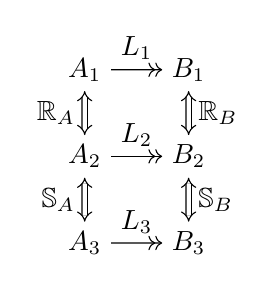
\begin{tikzpicture}[baseline=0.6mm,xscale=0.66,yscale=0.55]
    \node (A1) at (-1,  2) {$A_1$};
    \node (A2) at (-1,  0) {$A_2$};
    \node (A3) at (-1, -2) {$A_3$};
    \node (B1) at ( 1,  2) {$B_1$};
    \node (B2) at ( 1,  0) {$B_2$};
    \node (B3) at ( 1, -2) {$B_3$};
    \draw (A1) edge[->>] node[auto] {$L_1$} (B1);
    \draw (A2) edge[->>] node[auto] {$L_2$} (B2);
    \draw (A3) edge[->>] node[auto] {$L_3$} (B3);
    \begin{scope}[double equal sign distance, {Implies[]}-{Implies[]}]
      \draw (A1) edge[double] node[auto,swap] {$\mathbb{R}_A$} (A2);
      \draw (B1) edge[double] node[auto] {$\mathbb{R}_B$} (B2);
      \draw (A2) edge[double] node[auto,swap] {$\mathbb{S}_A$} (A3);
      \draw (B2) edge[double] node[auto] {$\mathbb{S}_B$} (B3);
    \end{scope}
  \end{tikzpicture}
  $
  \caption{Simulation identity and vertical composition}
  \label{fig:simcomp}
\end{figure}
%}}}

%}}}

%}}}


\paragraph*{Task 1a: Add support for unused-globals with better symbol table manipulation.}
blah blah blah.

\paragraph*{Task 1b: Add support for first-class code pointers.}
blah blah blah.

\paragraph*{Task 1c: Extend CompCertO to support multiple backends; and port it to the latest realese.}
blah blah blah.


\bibliographystyle{alpha}
\bibliography{references}

\end{document}

